%%% subsection
\subsection{Process 3: Signal Scheduler }
\label{subsec:process_3} 

Signal scheduling is the third process run by Traffic Control Unit (TCU).  The behavior of this process can be grouped into two state, Idle Signal Scheduling state and ROW emergency state as visualized in Figure \ref{img:process_3_state_machine}. In Idle Signal Scheduling state, the sequence of Right of Way (ROW) is fixed as depict in Figure \ref{img:process_3_internal_state_machine}. 

%%% image process 3 state machine
\begin{figure}[ht]
    \centering
    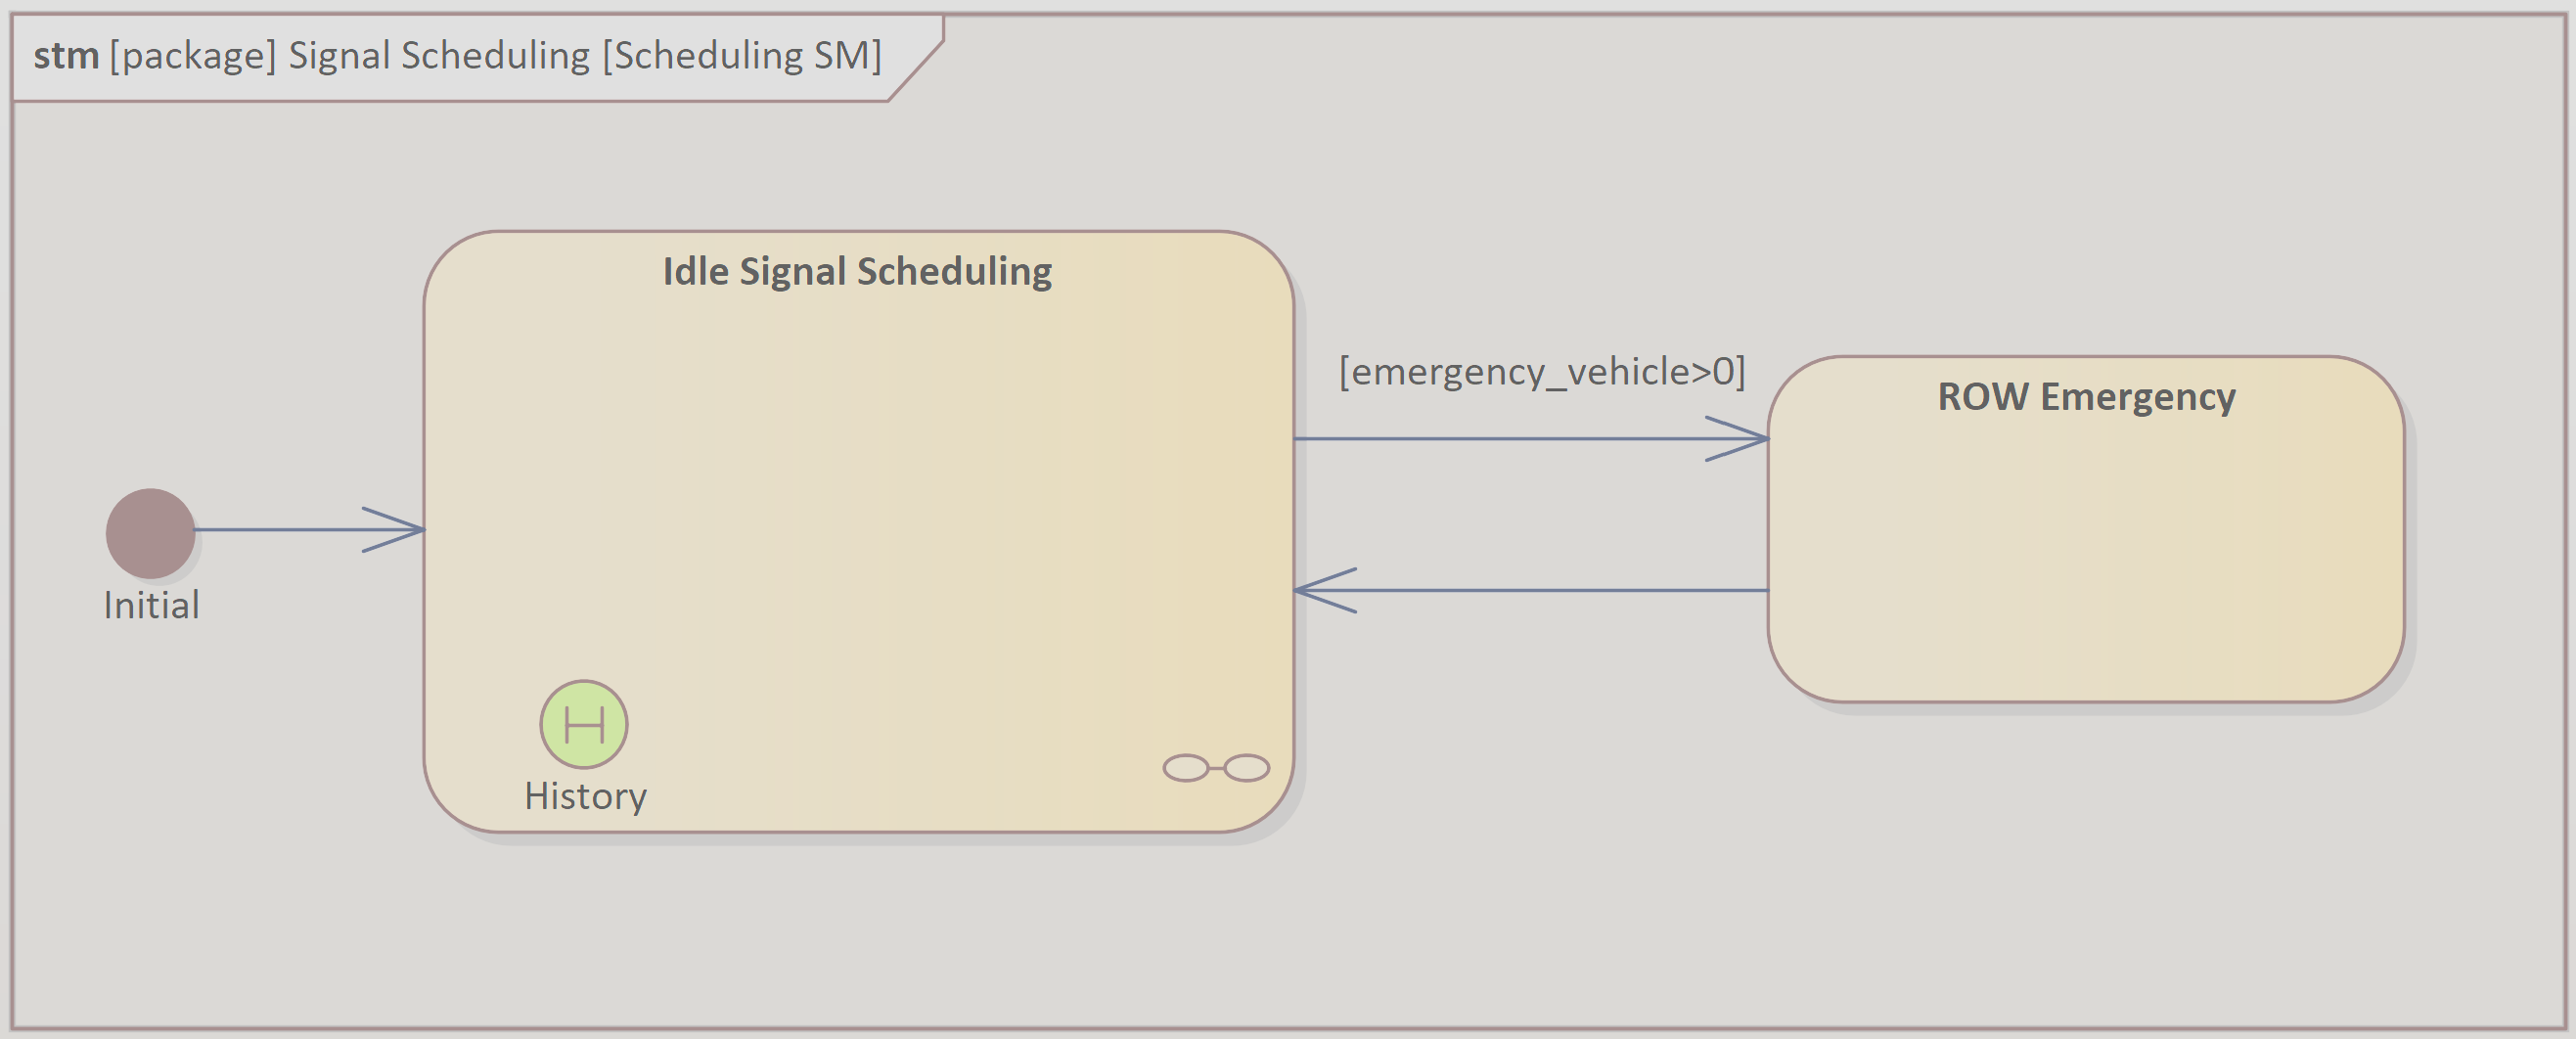
\includegraphics[width=0.5\textwidth]{images/process_3_state_machine.png}
    \caption{Signal Scheduling Process }
    \label{img:process_3_state_machine}
\end{figure}


Whenever the value of emergency vehicle is greater the 1, the process will change its state to ROW Emergency state. The variable is a global variable that is updated by Emergency Response process as explained in section \ref{subsec:process_2}. In ROW Emergency state, the process will change the ROW to the one that has emergency vehicle. For now, the duration for the process shall remain in the state within a fixed duration and shall turn back to Idle Signal Scheduling state.

%%% image internal state machine
\begin{figure}[ht]
    \centering
    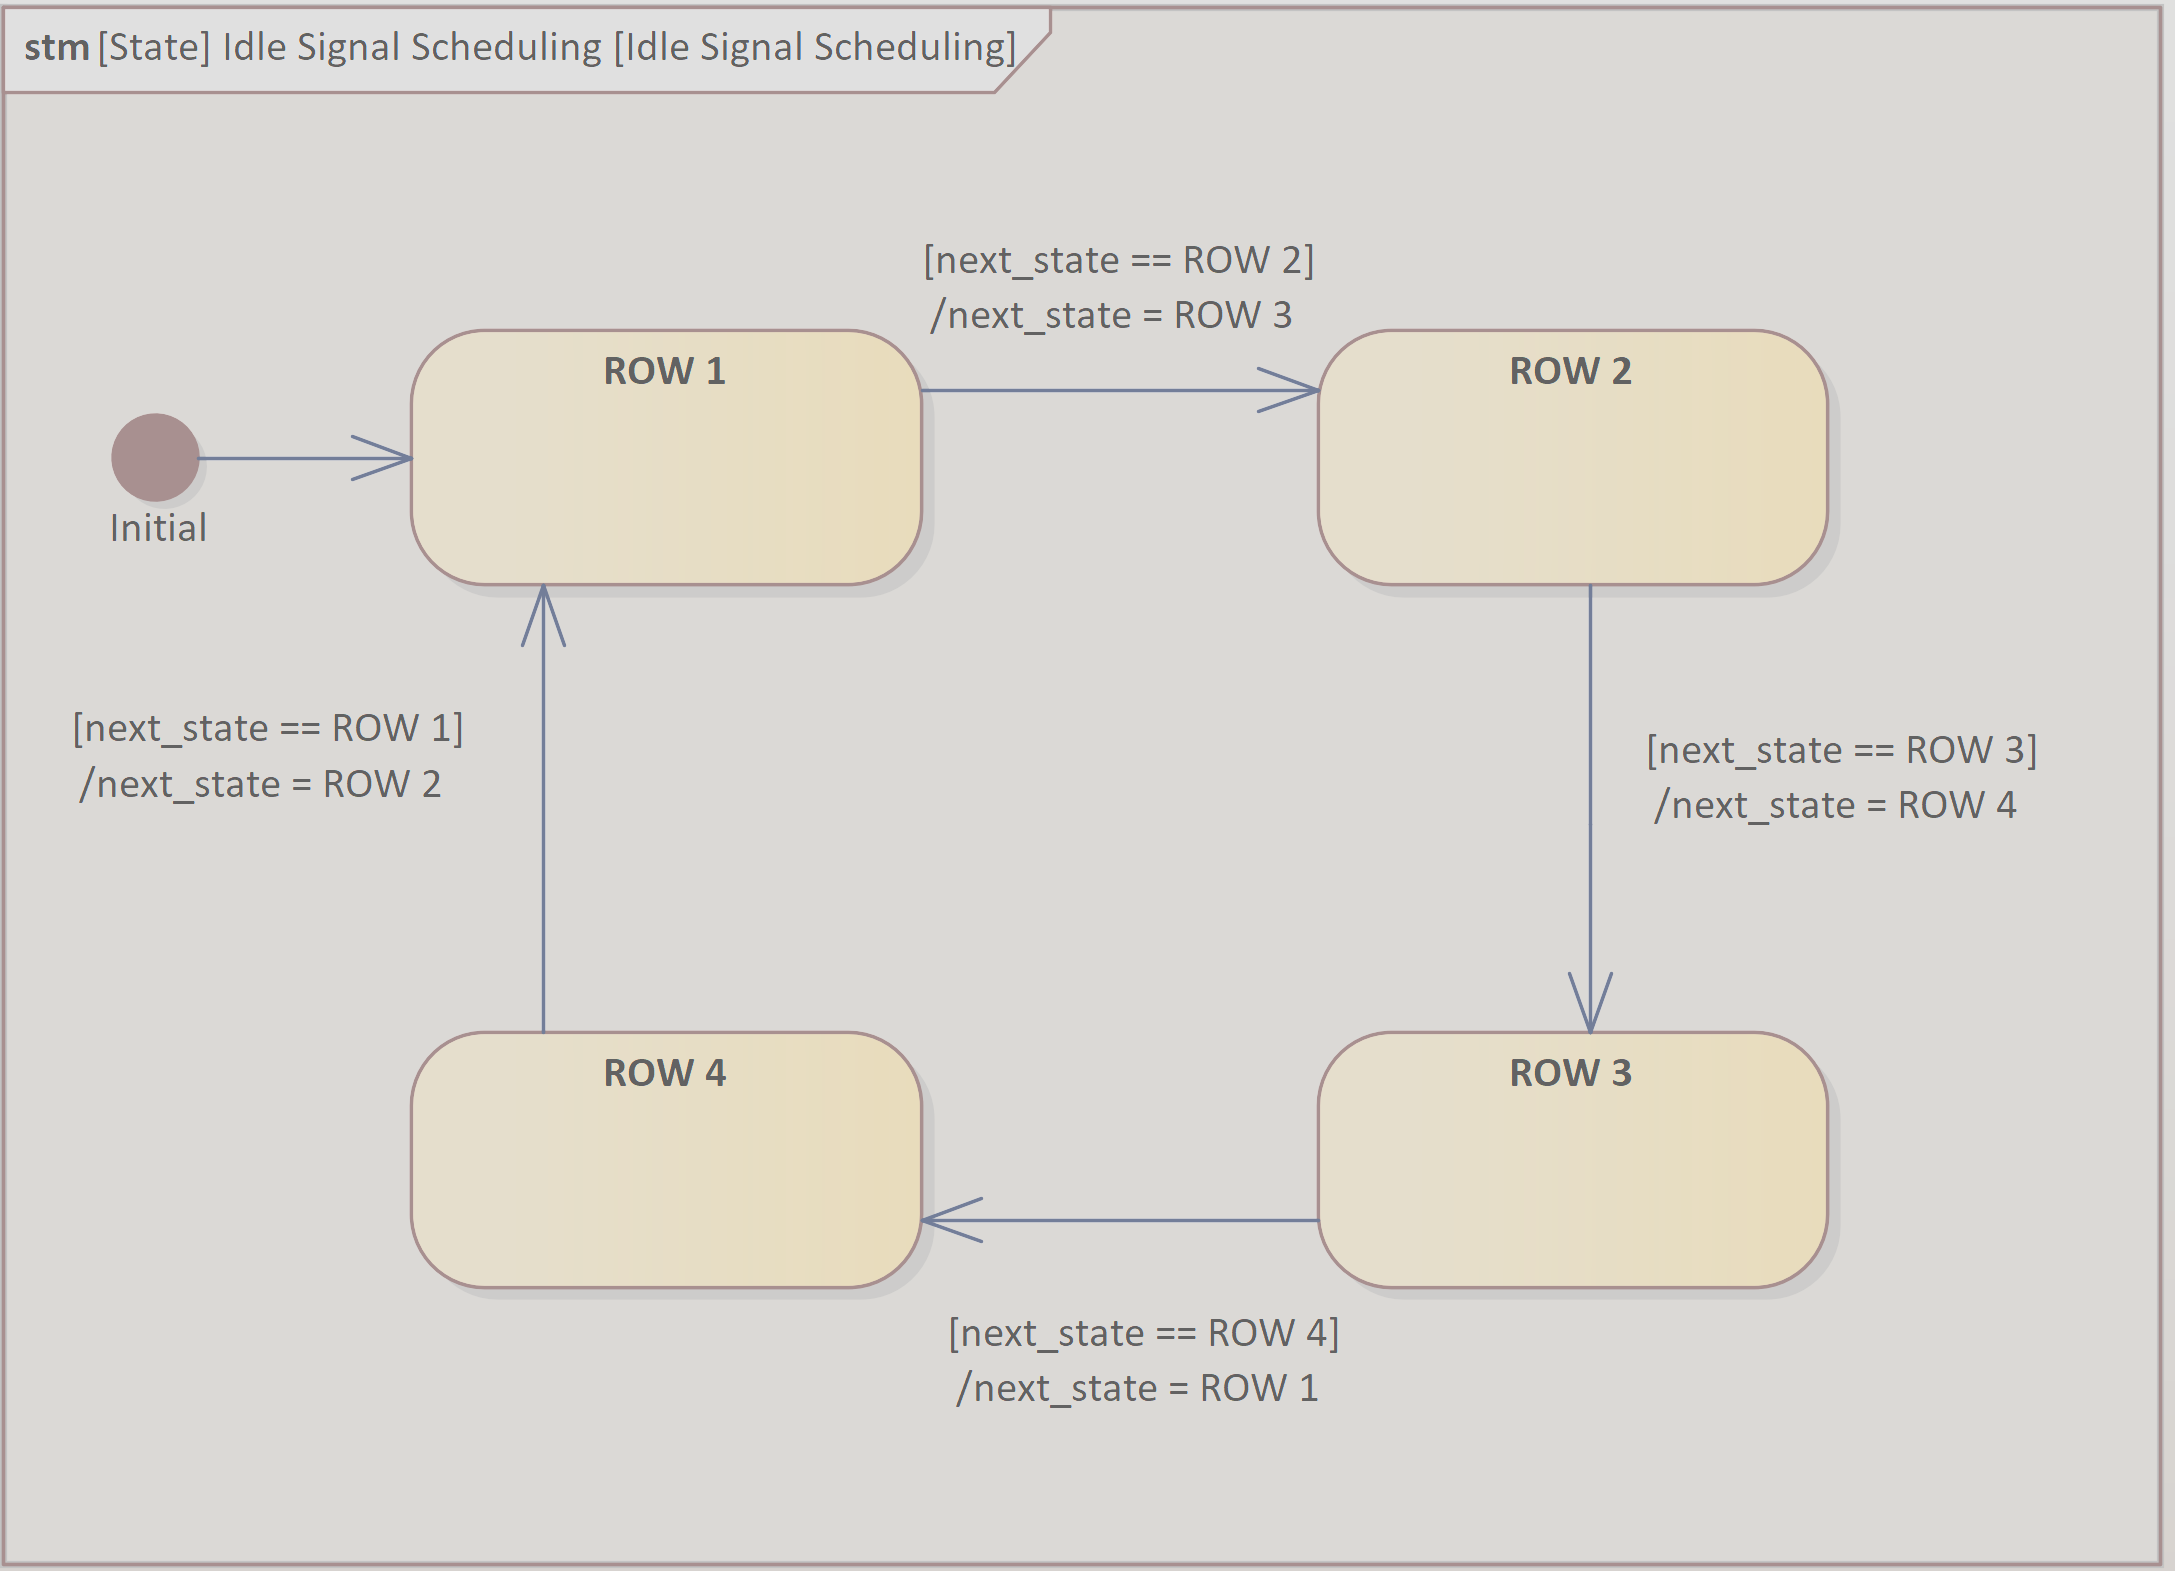
\includegraphics[width=0.45\textwidth]{images/process_3_internal_state_machine.png}
    \caption{Internal states of idle signal scheduling states}
    \label{img:process_3_internal_state_machine}
\end{figure}

Since Idle Signal Scheduling state is a history state, the process will back to previous ROW. This is to allow fairness between the ROWs. The process have the same procedure in every state even in ROW Emergency state because the state have fixed duration. The procedure is illustrated in Figure \ref{img:process_3_activity}. It shows that the bus input is also a parameter used by the process that were explained in section \ref{subsec:process_1}.

The TCU first updates its clock.Simultaneously, it actively monitors for the presence of an emergency state. If an emergency state is detected, the TCU proceeds to validate it. If the emergency state is valid, the TCU halts signal scheduling. In case the emergency state is invalid, the TCU concludes the emergency procedure and smoothly transitions back to the next appropriate state. When no emergency state is identified, the TCU proceeds to the next phase of validation. The TCU continues to validate its current state, and checking for duration extension or emergency input. If an emergency input is detected during this check, the TCU promptly shifts to the emergency state. In the absence of an emergency input, the TCU smoothly transitions to the next appropriate state in the sequence.
Following state transition, the TCU re-evaluates the validity of its current state. If the current state is found to be valid, the TCU progresses to the subsequent state, updating the signal accordingly. In cases where the current state is invalidated, the TCU proceeds to wait.
%%% image process 3 activity
\begin{figure}[h]
    \centering
    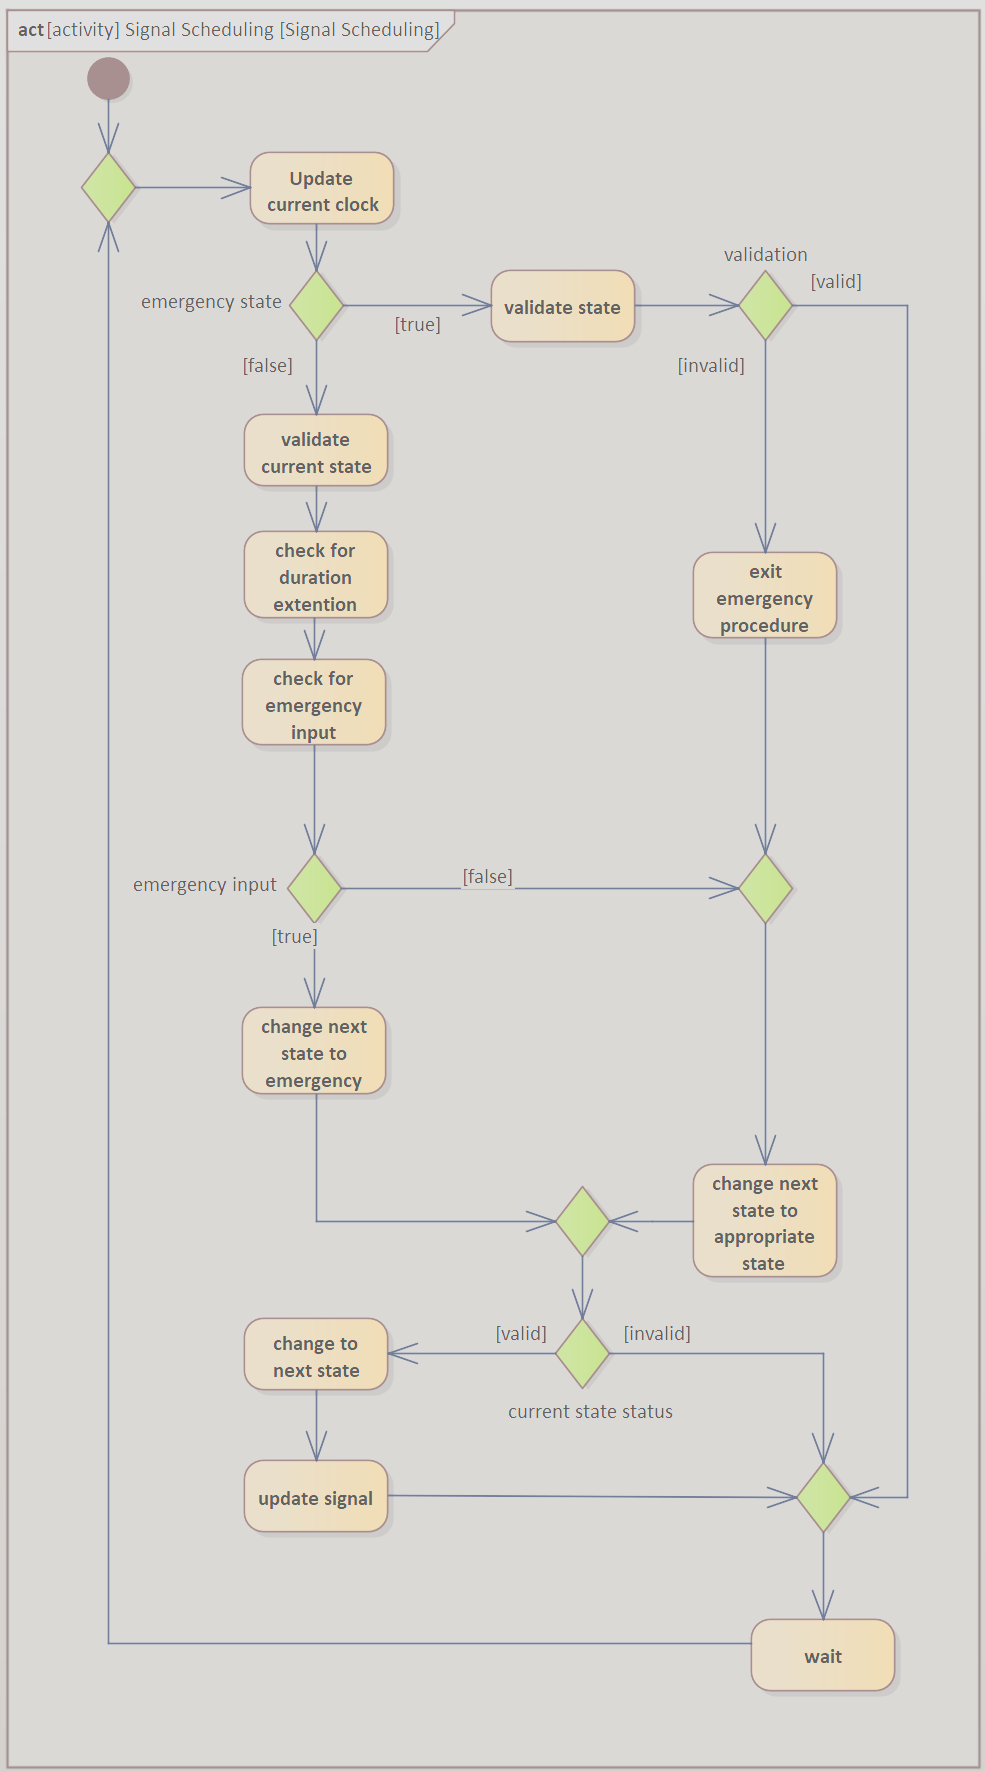
\includegraphics[width=0.3\textwidth]{images/process_3_activity.png}
    \caption{Signal scheduling process’ activity }
    \label{img:process_3_activity}
\end{figure}

In the next section, how these processes are executed in concurrent way on a chosen platform so that the system shall behave in predicted manner are explained.
